%\documentclass{article}
%\usepackage{graphicx,subfigure}
%\begin{document}

\begin{figure}[!h]
  \centering
  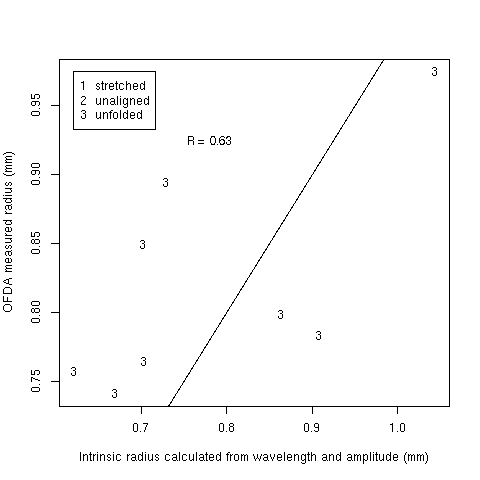
\includegraphics[width=1.0\textwidth]{figwaradthetaunfoldsfbase.png}
%   figwaradthetaunfoldsfbase.png is original 
  \caption{Intrinsic radius of curvature calculated from wavelength and amplitude measured by the SF technique on the base region of each staple, plotted against OFDA measured radius of curvature for unfolded wools only. Each point is a sheep mean for the base region.}
  \label{fig:waradthetaunfoldsfbase}
\end{figure}

%\end{document}

